\chapter{Considerações}\label{cap:definitions}

Para exemplificação dos cálculos foi proposta uma geometria conhecida contendo todas as medidas necessárias e também condições do ambiente onde essa geometria estará, com estes dados tornam se possíveis a criação de modelos puramentes numéricos.

\begin{figure}[h]
    \centering
    \caption{Geometria da peça proposta.}
    \label{fig:geometry}
    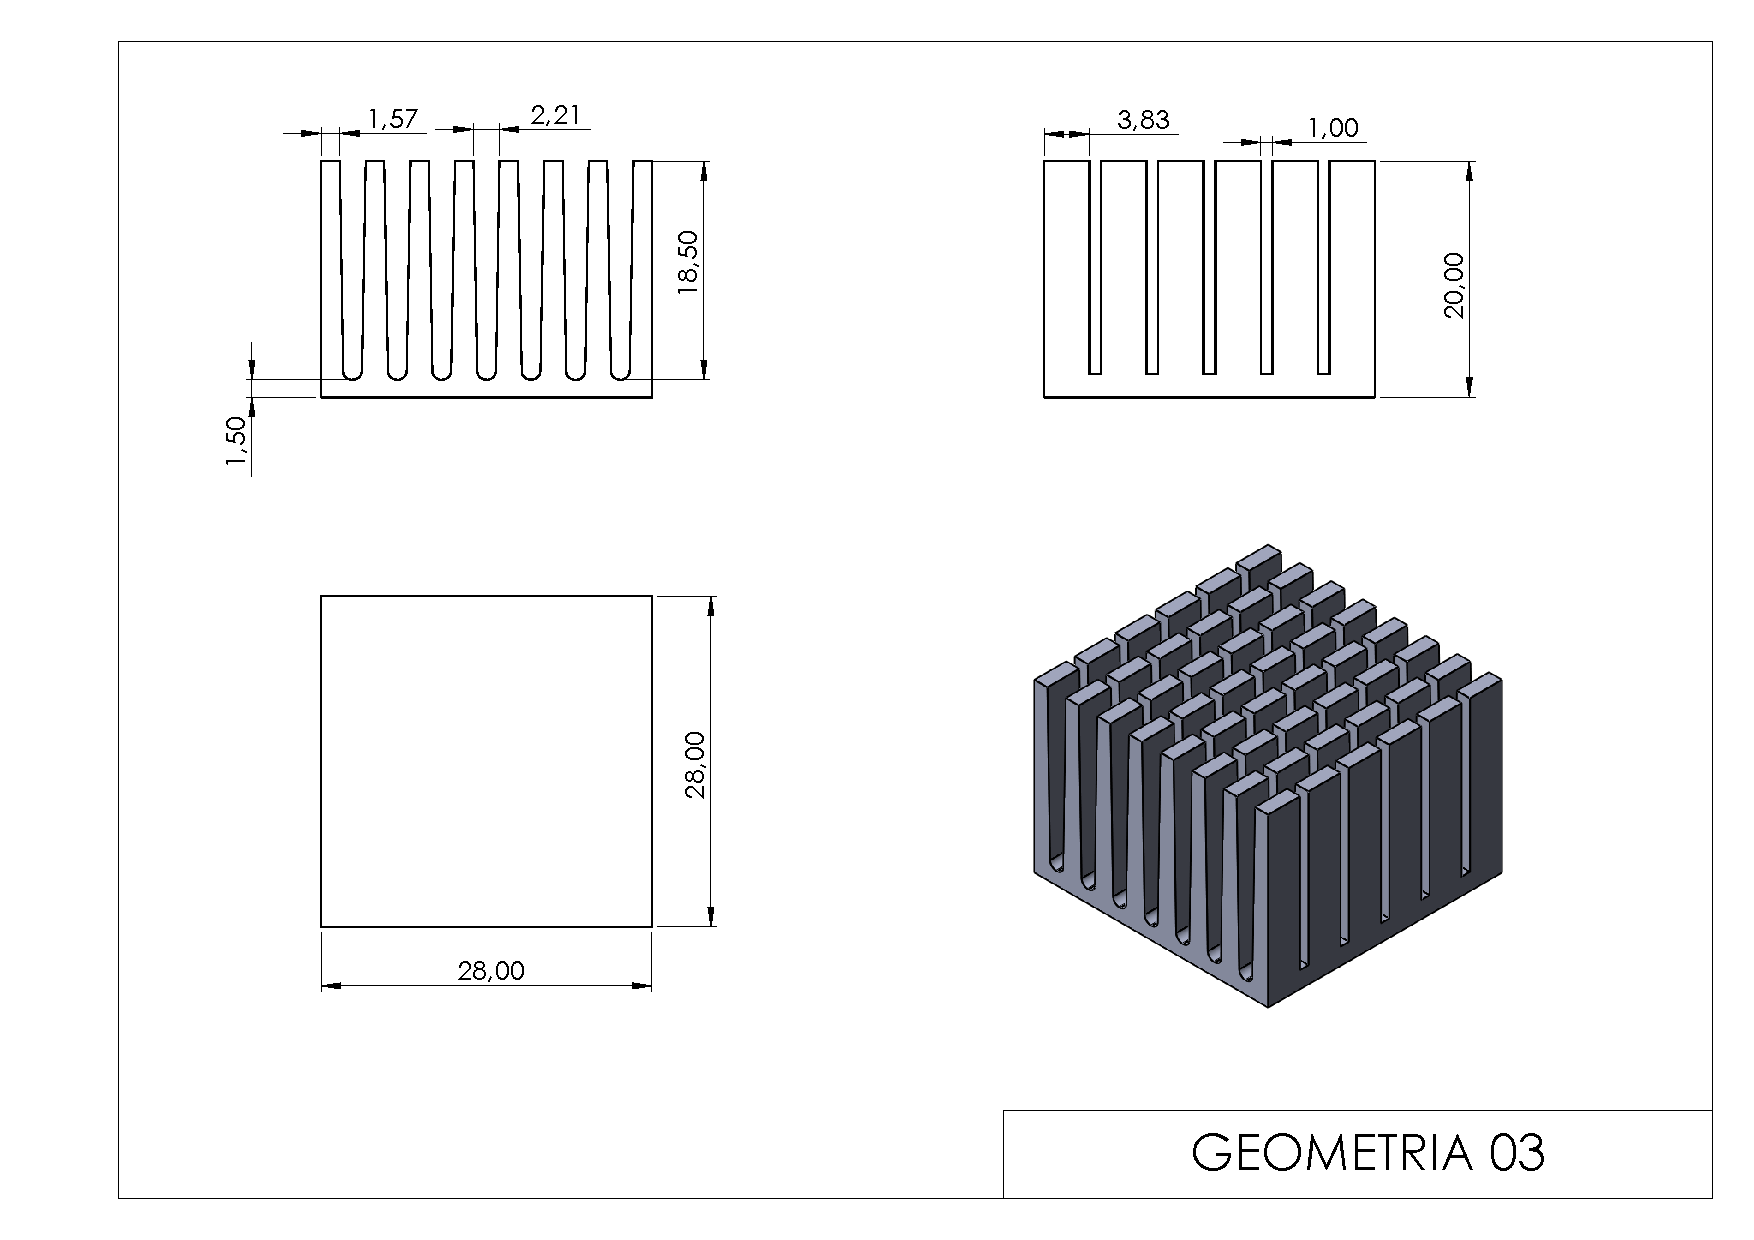
\includegraphics[width=15cm]{figuras/geometria.pdf}
    \fonte{\cite{antoniettiGeo}}
\end{figure}

Consideramos que a peça proposta será feita de alumínio, pelo fato do material ter um preço mais acessível e ter uma boa condução térmica, sendo amplamente utilizado na indústria para esse mesmo propósito.

\begin{figure}[h]
    \centering
    \caption{Tabela propriedades termofísicas de sólidos metálicos selecionados.}
    \label{fig:metalProps}
    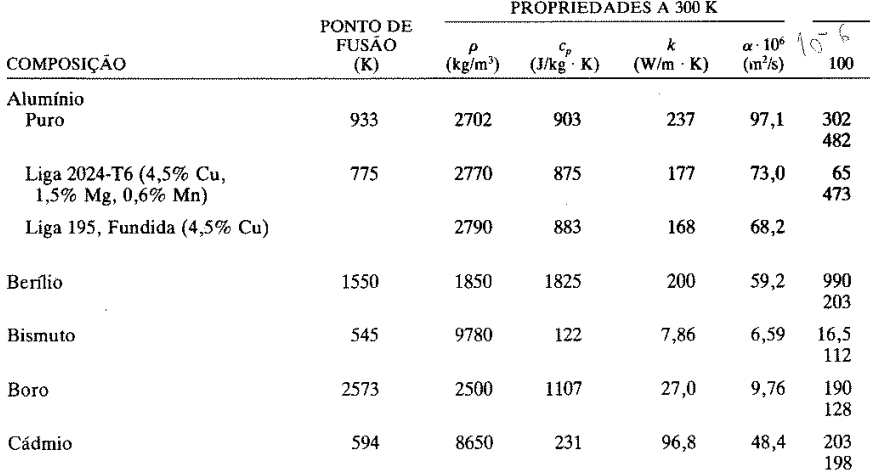
\includegraphics[width=14cm]{figuras/metalProps.jpg}
    \fonte{\citeonline{uspTabelasTermodinamicas}}
\end{figure}

Outras condições do funcionamento da condução térmica também foram pré-determinadas, sendo elas:

\begin{itemize}[leftmargin=2cm]
    \item Regime estacionário;
    \item Condutividade térmica constante;
    \item Radiação na superfície desprezível;
    \item Efeito de geração de calor ausentes;
    \item Coeficiente de transferência de calor h uniforme ao longo da superfície;
    \item Condições unidimensional na direção x;
    \item Transferência de calor por convecção.
\end{itemize}


\begin{table}[h]
    \ABNTEXfontereduzida
    \centering
    \caption{Grandezas fornecidas}
    \label{tab:grandezasFornecidas}
    \begin{tabular}{c c l}\toprule
        Grandeza    & Valor                                      & Descrição                                           \\
        \toprule
        k           & \SI{237}{\watt\per\meter\per\kelvin}       & Condutividade térmica do material - Alumínio        \\
        h           & \SI{20}{\watt\per\square\meter\per\kelvin} & Coeficiente de transferencia de calor por convecção \\
        T1          & \SI{110}\degreeCelsius                     & Temperatura da superficie                           \\
        T\(\infty\) & \SI{30}\degreeCelsius                      & Temperatura do ar ambiente                          \\
        Eb          & 0,0015 \SI{}{\meter}                       & Espessura da base                                   \\
        Lb          & 0,028 \SI{}{\meter}                        & Largura da base                                     \\
        Wb          & 0,028 \SI{}{\meter}                        & Profundidade da base                                \\
        ta          & 0,00157 \SI{}{\meter}                      & Espessura da aleta                                  \\
        La          & 0,0185 \SI{}{\meter}                       & Distância da base até na ponta da aleta             \\
        L total     & 0,02 \SI{}{\meter}                         & Altura total da peça                                \\
        Wa          & 0,00383 \SI{}{\meter}                      & Profundidade da aleta                               \\
        N           & 48un                                       & Quantidade de aletas                                \\
        e1          & 0,001 \SI{}{\meter}                        & Espaço entre as aletas pela frente                  \\
        e2          & 0,00221 \SI{}{\meter}                      & Espaço entre as aletas pelo lado                    \\
        \bottomrule
    \end{tabular}
    \fonteproprioautor
\end{table}